\documentclass[a4paper,11pt,french]{report}
 \usepackage[utf8]{inputenc} %latin9 ou1
 \usepackage[T1]{fontenc}
 \usepackage[normalem]{ulem}
 \usepackage[letterpaper]{geometry}
 \usepackage{lmodern} %fonte latin modern
 \usepackage[francais]{babel}
 \usepackage{verbatim}
 \usepackage{graphicx}
 \usepackage{subfig}
 \usepackage{multicol}
 \usepackage{hyperref}
 \hypersetup{colorlinks=true,linkcolor=blue,urlcolor=red}
 \usepackage{varioref}
 \usepackage{lettrine}
%\usepackage[letterpaper]{geometry}
%\geometry{verbose,tmargin=3cm,bmargin=3cm,lmargin=3cm}
%\usepackage{varioref}

%\usepackage{babel}
\usepackage{fancyhdr}
\cfoot{Page \thepage}
\pagestyle{fancy}

\usepackage{listings}   % need for code encapsulation
\lstset{
	language=Python,
	numbers=left, numberstyle=\tiny, stepnumber=1, numbersep=7pt,
	morekeywords={%
    %%% BOUCLE, TEST & Co.
      if, elif, then, else, and, or, until, yield,repeat,
    %%% IMPORT & Co.
      import, from, package,
    %%% FONCTIONS NUMERIQUES
      cos, sin, tan, acos, asin, atan,
    %%% CONSTANTES
      pi, True, False,
    %%% Types .
      Int, String, Array, Integer, 
    %%% Mots-Clefs supp.
      object, class, protected, public, private, final, val, var, new, ?, !
    },
    sensitive=true,
    morecomment=[l]{\#},
	keywordstyle=\bfseries\emph,
	breaklines=true,	
	frameround=fttt,
	basicstyle= \mdseries\scriptsize }
%\lstset{language=bash,basicstyle=\scriptsize,commentstyle=\small\itshape,stringstyle=\ttfamily,numbers=left,numberstyle=\tiny,stepnumber=1,showstringspaces=false}
	
% Commandes personnelles
\def\clap#1{\hbox to 0pt{\hss #1\hss}} % Une commande sembleble  \rlap ou \llap, mais centrant son argument
\def\ligne#1{\hbox to \hsize{\vbox{\centering #1}}} % Une commande centrant son contenu ( utiliser en mode vertical)
% Une comande qui met son premier argument  gauche, le second au 
% milieu et le dernier  droite, la premire ligne ce chacune de ces
% trois boites coincidant
\def\haut#1#2#3{\hbox to \hsize{\rlap{\vtop{\raggedright #1}}\hss \clap{\vtop{\centering #2}} \hss \llap{\vtop{\raggedleft #3}}}}%
% Idem, mais cette fois-ci, c'est la dernire ligne
\def\bas#1#2#3{\hbox to \hsize{\rlap{\vbox{\raggedright #1}} \hss \clap{\vbox{\centering #2}} \hss \llap{\vbox{\raggedleft #3}}}}%
    
    
% La commande \maketitle
\makeatletter
	\def\maketitle{%
	  \thispagestyle{empty}\vbox to \vsize{%
		\vspace{3cm} \ligne{\Huge \textsc \@title}
		\vspace{7mm} \ligne{\Large \@subtitle}
		\vspace{1cm} \haut{Supervisé par \@supervisor}{}{\@follower}
		\vspace{3mm}\hrule
		\vfill
		\haut{}{Jérôme \textsc{Gazel}}{}
		\haut{}{$\&$}{}
		\haut{}{Clément \textsc{Schiano de Colella}}{}
		\vspace{3cm}
		\bas{}{\@location, \@date}{}
		}%
	  %\cleardoublepage
	  }

	% Les commandes permettant de dfinir la date, le lieu, etc.
	\def\date#1{\def\@date{#1}}
	\def\title#1{\def\@title{#1}}
	\def\subtitle#1{\def\@subtitle{#1}}
	\def\location#1{\def\@location{#1}}
	\def\blurb#1{\def\@blurb{#1}}
	\def\supervisor#1{\def\@supervisor{#1}}
	\def\follower#1{\def\@follower{#1}}
	\def\email#1{\def\@email{\small{#1}}}
	% Valeurs par dfaut
	\date{\today}
\makeatother


  \title{Programmation Concurrentielle}
  \subtitle{Communicating Scala Objects\\Java Communicating Sequential Processes}
  \location{Nantes}
  \lhead{\itshape PAPPLE - 2011}
  \supervisor{M.\ Olivier \textsc{Roux}}
  \follower{\'Ecole Centrale de Nantes}

\begin{document}
\maketitle
\tableofcontents

\newpage

\lettrine{L}{'importance} de la programmation concurrente n'a cessé de croître depuis quelques années. Sa connaissance et sa maîtrise deviendra à terme une nécessité pour tous les développeurs au regard du besoin de parallélisation des tâches.\\
Pour mettre en place une programmation concurrente, on peut d'ores et déjà utiliser \textsc{CSP}. Imaginé par Hoare, cet algèbre de processus permet de modéliser les différentes interactions entre systèmes. Ce langage a connu plusieurs implémentations pour les principaux langages de programmation et notamment pour Java et Scala.\\

Notre travail a donc consisté à prendre en main ces bibliotèques, voire le langage pour Scala, puisque nous connaissions peu ce langage avant ce projet.\\
Nous exposerons donc leur mise en place. Les principales caractéristiques de ces implémentations seront décrites, puis nous exposerons les programmes classiques de la programmation concurrente décrits à l'aide de ces implémentations. Enfin, nous dresserons un bilan de notre travail.\\

\chapter{Notions générales via CSP}

\lettrine{A}{fin de} rendre ce rapport indépendant et utilisable par le plus grand nombre, nous avons fait le choix de faire ici un rapide aperçu de CSP, afin que le lecteur puisse comprendre les mécanismes mis en place dans la suite. Pour faire cette présentation, nous nous sommes principalement inspiré du cours Parallélisme et Systèmes Répartis d'Olivier Roux \cite{pasyr}. \\
Hoare dans un article devenu célèbre présente le CSP (Communicating Sequential Processes). Il s'agit d'un langage impératif, parallèle, avec des communications par échanges synchrones de message.

\section{Notion de rendez-vous}
Le CSP utilise des commandes d'entrées et de sortie pour synchroniser ses messages. Pour transmettre un message entre un producteur et un consommateur, par exemple x, on utilise :

\begin{lstlisting}[frame=trBL]
P:: Q ! M(x)
Q:: P ? M(y)
\end{lstlisting}
 \begin{itemize}
 \item P : proc. originaire
 \item Q : proc. destinataire,
 \item M : identificateur de message
 \item x : contenu du message
 \end{itemize}
 
 \section{Notion de garde et commande gardée}
 Voici la forme usuelle utilisant la garde et la commande gardée :
 
 \begin{lstlisting}[frame=trBL]
<commande gardee> ::= <garde> -> <suite d instructions>
<garde> ::= <CB>, <CES>
\end{lstlisting}

En fonction des gardes, on a les conséquences suivantes :
\begin{itemize}
\item fausse : CB fausse ou correspondant de la CES inexistant ou
mort $\rightarrow$ échec de la commande gardée
\item vraie : CB vraie et correspondant de la CES prêt à échanger $\rightarrow$ communication ET exécution de la suite d’instructions qui suit
la garde
\item neutre : CB vraie et correspondant de la CES indisponible $\rightarrow$
attente (de communication)
\end{itemize}

On peut maintenant implémenter une sélective ou une répétitive.

\section{Sélective}
Sélective : choix indéterministe parmi toutes les gardes vraies,
attente si aucune n’est vraie, et échec de la sélective si toutes
sont fausses

 \begin{lstlisting}[frame=trBL]
[[
	(state=1) -> state:=state+1;
[]
	(state=1) -> state:=state-1;
]]
\end{lstlisting}

 \section{Répétivite}
 Idem de façon répétitive jusqu’à ce que toutes les
gardes soient fausses

\begin{lstlisting}[frame=trBL]
x:=1;
*[[
	(x<=N) -> imprimer(x); x++;
[]
	(x=N) -> skip;
]]
\end{lstlisting}




\part{Implémentation des différents langages}
\chapter[CSO]{Communicating Scala Objects -- CSO}
\begin{quotation}
\textit{\og CSO (Communicating Scala Objects) – a notationally convenient embedding of the essence of occam in a modern, generically typed, object-oriented programming language that is compiled to Java Virtual Machine (JVM) code.\fg}
\begin{flushright}
\textsc{Bernard Sufrin}
\end{flushright}
\end{quotation}
\bigskip
\section{Approche de Scala et de CSO}

\lettrine{S}{ous la} supervision de notre encadrant M.\ \textsc{Roux}, nous nous sommes penchés sur CSO -- Communcating Scala Objects. Ce language est une extension de Scala\footnote{Site officiel (en anglais) à l'adresse \url{http://www.scala-lang.org/}}, et permet d'implémenter tout algorithme de programmation concurrentielle.\\

Scala est un langage de programmation multi-paradigme conçu à l'École polytechnique fédérale de Lausanne (EPFL) pour exprimer les modèles de programmation courants dans une forme concise et élégante. Son nom vient de l'anglais Scalable language qui signifie à peu près \og langage adaptable \fg ou \og langage qui peut être mis à l'échelle \fg. Il peut en effet être vu comme un métalangage.
Scala, qui est un langage relativement jeune (2006), intègre les paradigmes de \emph{programmation orientée objet} et de \emph{programmation fonctionnelle}, avec un typage statique. Il concilie ainsi ces deux paradigmes habituellement opposés (à de rares exceptions près, telle que le langage OCaml) et offre au développeur la possibilité de choisir le paradigme le plus approprié à son problème (source \textsc{Wikipedia}).\\

Notre seule est unique source pour ce projet a été la publication du Dr.\ \textsc{Sufrin} \cite{cpa2008-cso}, qui trace un premier tutoriel de CSO, et qui fournit un exemple d'implémentation pour le jeu de la vie intitulé \og \emph{lyfe} \fg.\\

\subsection{Installation de Scala et de CSO}

La première étape est d'installer Scala et CSO sur notre machine. Première difficulté car très peu voire aucune documentation est disponible à ce sujet. 

\begin{quotation}
\textit{\og This task speaks for itself. If you find it hard to do this then you may find it impossible
to accomplish any of the subsequent tasks.\fg}
\begin{flushright}
\textsc{Bernard Sufrin}
\end{flushright}
\end{quotation}
Après deux semaines de recherche pour arriver à effectuer cette tâche, nous avons conçu un script \textsf{sh} pour les machines sous GNU/Linux.\\

\begin{lstlisting}[frame=trBL, language=bash, title={install\_{}cso.sh}]
#!/bin/bash
# Script pour installer CSO sur une machine sous GNU/Linux

wget http://www.scala-lang.org/downloads/distrib/files/scala-2.8.1.final.tgz

tar -xvzf scala-2.8.1.final.tgz
rm scala-2.8.1.final.tgz
mv scala-2.8.1.final ~/Scala

echo 'export SCALA_HOME="~/Scala"' >> ~/.bashrc
echo 'export PATH=$PATH:${SCALA_HOME}/bin' >> ~/.bashrc

mkdir ~/ScalaLocal

wget http://users.comlab.ox.ac.uk/bernard.sufrin/CSO/cso-sources-scala2.8.0.tgz
tar -xvf cso-sources-scala2.8.0.tgz
rm cso-sources-scala2.8.0.tgz

mv scalatasks.xml ~/ScalaLocal/

source ~/.bashrc
scala -version
ant jar

cp cso.jar ~/ScalaLocal
cp cswing.jar ~/ScalaLocal

echo "Installation CSO Terminee"
\end{lstlisting}
\subsection{Lyfe}
Le jeu de la vie, automate cellulaire imaginé par John Horton Conway en 1970, est probablement, à l’heure actuelle, le plus connu de tous les automates cellulaires.\\
\emph{Lyfe} se déroule sur une grille à deux dimensions en $10\times 10$ ou $15\times 15$, dont les cases -- qu’on appelle des \og cellules \fg, par analogie avec les cellules vivantes -- peuvent prendre deux états distincts : \emph{vivantes} ou \emph{mortes}.\\

Notre précédent script a télécharger directement le jeu \emph{Lyfe} dans le répertoire courant, sous le nom de \textbf{CSwing}.\\
Pour l'exécuter, il suffit maintenant d'effectuer les deux commandes :

\begin{verbatim}
ant jar
ant lyfe
\end{verbatim}

Nous obtenons une interface graphique agréable, où les clics de la souris permet de changer l'état d'une cellule (\emph{cf.} Figure~\vref{fig:lyfe}). L'initialisation de logiciel se fait avec une première configuration des cellules (\emph{cf.}~\vref{fig:lyfe-a}); un premier clic sur une cellule lancera le programme (\emph{cf.}~\vref{fig:lyfe-b}).

\begin{figure}[htp]
  \centering
  \subfloat[Lancement du programme Lyfe (configuration initiale)]{\label{fig:lyfe-a}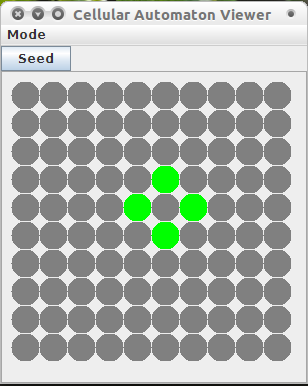
\includegraphics[scale=0.5]{Lyfe.png}} 
  \vspace{1pt}               
  \subfloat[Après une première configuration et plusieurs itérations (anti-aliasing activé)]{\label{fig:lyfe-b}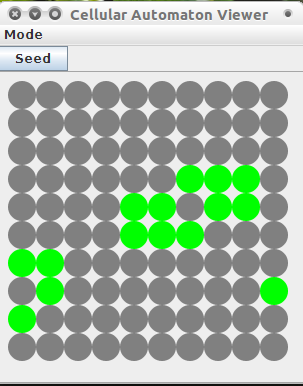
\includegraphics[scale=0.5]{Lyfe2.png}}
  \caption{Programme Lyfe, proposé par Dr.\ \textsc{Sufrin}}
  \label{fig:lyfe}
\end{figure}

\subsection[Vers les algorithmes classiques...]{Vers les algorithmes classiques... : Utilisation de \textsf{ant} et premiers essais}

Après avoir construit un fichier \textsf{buid.xml} capable de compiler, nettoyer, lancer le programme en adjoignant les bonnes ressources via une simple commande, puis avoir saisi la syntaxe nécessaire d'abord à Scala, puis à CSO, les programmes 'producteur-consommateur' et 'lecteur-écrivain'étaient l'un des objectifs de notre projet.\\

Cependant, après des résultats infructueux, il semblerait que notre équipe ait mis à jour un problème relevant du comportement de CSO vis-à-vis des processus concurrents. En effet, leur ordre d'arrivée dépend de leur position dans la sélective; ce qui ne devrait pas être le cas.\\ 

En d'autres termes, les processus ne s'executent que si l'un d'entre eux se finit (à la manière séquentielle d'un \textsc{Fifo}). Voici quelques exemples qui nous ont amenés à cette conclusion.

\subsubsection{Illustration du problème}

Pour illustrer ces propos, considérons le programme suivant \textsf{HelloWorld} qui lancent plusieurs procesus en parallèle, chacun ayant soit la tâche d'afficher "Hello" soit d'afficher "World".\\
La syntaxe-clef ici est la double-barre ||, qui permet de décrire une sélective, mais donne aussi la possiblité via l'opérateur \textsf{for} de lancer \textit{n} processus en parallèle.\\
Cette syntaxe est notamment décrite dans le rapport émis par Dr.\ \textsc{Sufrin}\footnote{Page personnelle de Bernard \textsc{Sufrin} à l'adresse \url{http://users.comlab.ox.ac.uk/bernard.sufrin/}} \cite{cpa2008-cso}, ainsi que dans le programme Lyfe qu'il met à disposition sur son site internet.
\medskip

\begin{lstlisting}[frame=trBL]
package helloworld
import ox.CSO._

object Hello_Par {

    val NP = 3
    val NC = 4
    
    def main( args: Array[String] ) {
  
        println("Debut du programme HelloWord Par :")
        ( 
           || ( for (i <- 0 until NP) yield Hello(i) )
        || 
           || ( for (i <- 0 until NC) yield World(i) )
        )()
        
    }


    def Hello( i: Int ) : PROC={
    	say("Hello" + i)
    } 

    def World( i: Int ) : PROC={
    	say("World" + i)
    }

    def say( word: String ) {
      println(word)
    }  
}
\end{lstlisting}

Les résultats obtenus avec cette syntaxe sont présentés dans la figure~\vref{fig:1HW}.

\begin{figure}[h]
\centering
\begin{multicols}{2}
\begin{lstlisting}[frame=trBL]
     [exec] Debut :
     [exec] Hello0
     [exec] Hello1
     [exec] World3
     [exec] World2
     [exec] World0
     [exec] World1
     [exec] Hello2
     [exec] Debut :
     [exec] Hello2
     [exec] Hello1
     [exec] Hello0
     [exec] World3
     [exec] World2
     [exec] World0
     [exec] World1
     [exec] Debut  :
     [exec] Hello2
     [exec] Hello0
     [exec] Hello1
     [exec] World3
     [exec] World0
     [exec] World2
     [exec] World1
     [exec] Debut  :
     [exec] Hello2
     [exec] Hello0
     [exec] Hello1
     [exec] World3
     [exec] World2
     [exec] World1
     [exec] World0
     [exec] Debut  :
     [exec] Hello2
     [exec] Hello1
     [exec] Hello0
     [exec] World3
     [exec] World2
     [exec] World0
     [exec] World1
     [exec] Debut  :
     [exec] Hello2
     [exec] Hello1
     [exec] Hello0
     [exec] World3
     [exec] World2
     [exec] World0
     [exec] World1
     [exec] Debut  :
     [exec] Hello2
     [exec] Hello0
     [exec] Hello1
     [exec] World3
     [exec] World1
     [exec] World0
     [exec] World2
     [exec] Debut  :
     [exec] Hello2
     [exec] Hello0
     [exec] Hello1
     [exec] World3
     [exec] World2
     [exec] World1
     [exec] World0
     [exec] Debut  :
     [exec] Hello2
     [exec] World2
     [exec] Hello1
     [exec] Hello0
     [exec] World3
     [exec] World0
     [exec] World1
     [exec] Debut  :
     [exec] Hello2
     [exec] Hello0
     [exec] Hello1
     [exec] World3
     [exec] World2
     [exec] World0
     [exec] World1
     [exec] Debut  :
     [exec] Hello2
     [exec] Hello1
     [exec] Hello0
     [exec] World3
     [exec] World2
     [exec] World0
     [exec] World1
     [exec] Debut  :
     [exec] Hello2
     [exec] Hello1
     [exec] Hello0
     [exec] World3
     [exec] World2
     [exec] World0
     [exec] World1
     [exec] Debut  :
     [exec] Hello2
     [exec] Hello0
     [exec] Hello1
     [exec] World3
     [exec] World2
     [exec] World0
     [exec] World1
\end{lstlisting}
\end{multicols}
\caption{Résultat du premier HelloWorld en programmation concurrente}
\label{fig:1HW}
\end{figure}

On remarque bien que les processus dépendent de leur place dans la sélective, et leur ordre est même (sauf exceptions) quasiment le même.

\subsubsection{Pour aller plus loin}

Ce problème peut certes paraître minime. L'essentiel est bien sûr que l'ensemble des processus se comporte comme s'il tournait en parallèle.\\ Ici tout porte à croire que c'est cependant le cas. Mais un autre exemple démontre la séquencialité de l'exécution (\emph{cf.} l'encadré suivant)

\begin{lstlisting}[frame=trBL, title={Contre-exemple démontrant la séquentialité de l'exécution}]
package gazel_schiano_cso
import ox.CSO._

object ProdCons {
    val NP = 4
    val NC = 1
    val N = 4
    var enVie = true

    val left, mon, right = ManyMany[String]

    def main( args: Array[String] ) {
        
        println("Debut du programme Producteur-Consommateur")
        ( 
           || ( for (i <- 0 until NP) yield Producteur(i, mon) )
        || 
           || ( for (i <- 0 until NC) yield Consommateur(i, mon) )
        || 
           Buffer(mon) 
        )()
    }
\end{lstlisting}
\begin{lstlisting}[frame=trBL, title={Contre-exemple, suite : Producteur}, firstnumber=last]    
    
    def Producteur(i : Int, out : ![String]) : PROC = {
        var nb = 0
        var message = ""
        println("Creation d'un producteur (" + i + ").")
        
        //repeat(enVie) {
            println("   Boucle Producteur -- Objet numero " + nb)
            sleep(i)
            message = "Objet numero " + nb
            println(message)
            mon ! message
            out ! message
            println("Production " + i + " : " + message)
            nb = nb + 1
        //}
    }
\end{lstlisting}
\begin{lstlisting}[frame=trBL, title={Contre-exemple, suite : Consommateur et Buffer}, firstnumber=last]
    def Consommateur(i : Int, in : ?[String]) : PROC = {
        var k = 0
        println("Creation d'un consommateur (" + i + ") :: enVie? " + enVie)
        
        //repeat(enVie) {
            println("   Boucle Consommateur")
            in ? { message => 
                    {
                        mon ! message 
                        right! message 
                        println("Consommateur " + i + " : " + message)
                    } 
                }
            //sleep(500*i)
        //}
    }  
    

    def  Buffer( tuyau : ?[String] ) : PROC = {
        println("Entree Buffer")
        tuyau ? { v => {println(v)}}
    }
    
}
\end{lstlisting}

Ce qui donne ici à l'execution l'encadré \vref{fig:contreexemple-resultat}, qui se fige lors de l'attente de l'objet via le pipe.

\begin{figure}[h]
\begin{lstlisting}[frame=trBL]
     [exec] Debut du programme Producteur-Consommateur
     [exec] Creation d'un producteur (0).
     [exec]    Boucle Producteur -- Objet numero 0
     [exec] Objet numero 0
     [exec] Production 0 : Objet numero 0
     [exec] Creation d'un producteur (1).
     [exec]    Boucle Producteur -- Objet numero 0
     [exec] Objet numero 0
     [exec] Production 1 : Objet numero 0
     [exec] Creation d'un producteur (2).
     [exec]    Boucle Producteur -- Objet numero 0
     [exec] Objet numero 0
     [exec] Production 2 : Objet numero 0
     [exec] Creation d'un producteur (3).
     [exec]    Boucle Producteur -- Objet numero 0
     [exec] Objet numero 0
     [exec] Production 3 : Objet numero 0
     [exec] Creation d'un consommateur (0) :: enVie? true
     [exec]    Boucle Consommateur
\end{lstlisting}
\caption{Contre-exemple démontrant la séquentialité de l'exécution [Résultats]}
\label{fig:contreexemple-resultat}
\end{figure}

\paragraph{Constats} L'encha\^inement de l'instanciation se fait de manière séquentielle; d'abord en commençant par les porducteurs, puis par le consommateur.

\paragraph{Que se passe-t-il ?} Il est clair que l'instanciation se fait de manière séquentielle, et que le Buffer \textit{mon} n'exite pas encore. De ce fait, l'essai de l'envoi via le pipe vers \textit{mon} ne peut pas aboutir, et on aboutir à un interblocage...

\section{Premiers résultats}
\subsection{Instanciation}

Nous l'avons vu, le problème se situe au niveau de l'instanciation. Nous sommes passés à c\^oté d'un point important dans le langage Scala: la différenciation entre les \textsf{object} et les \textsf{class}.\\

Essayons d'écrire un classe, et de définir à l'intérieur une méthode \textsf{proc}:

\begin{lstlisting}[frame=trBL]
package helloworld
import ox.CSO._
import ox.Format._
import ox.cso.Components.{console}

object Hello_Pipe {

    var enVie = true

    val pipe = OneOne[String]

    def main( args: Array[String] ) {
        println("Debut du programme Hello_Pipe")
        var sender = new Sender(pipe)
        var receiver = new Receiver(pipe)
        ( 
           sender.process
        || 
           receiver.process
        )()
    }

    class Sender(out: ![String])
    {
        val process : PROC =
        { 
            println("Creation d'un sender")
            repeat 
            {
                var message = "Mon Objet"
                println(">> Envoi de \"" + message + "\"...")
                out!message
                sleep(500)
            }
        }  
    }

    class Receiver(in: ?[String])
    {
        val process : PROC =
        { 
            println("Creation d'un receiver")
            var message =""
            repeat 
            {
                message=in ?; 
                println("\"" + message + "\" recu.")
            }
         }  
    }   
}
\end{lstlisting}
\bigskip

Ce problème s'apparente à un algorithme de producteur-consommateur, car la production crée le message, tandis que la consommation l'affiche, tout cela via un pipe.\\
Le résultat obtenu est le suivant:


\begin{lstlisting}[frame=trBL]
Buildfile: /home/jerome/Documents/Pappl/git/CSO/HelloWorld/build.xml

pipe:
     [exec] Debut du programme Hello_Pipe
     [exec] Creation d'un sender
     [exec] Creation d'un receiver
     [exec] Envoi de "Mon Objet"... >>
     [exec] <<Mon Objet recu
     [exec] Envoi de "Mon Objet"... >>
     [exec] <<Mon Objet recu
     [exec] Envoi de "Mon Objet"... >>
     [exec] <<Mon Objet recu
     [exec] Envoi de "Mon Objet"... >>
     [exec] <<Mon Objet recu
\end{lstlisting}

\bigskip

\textbf{Constats} L'envoi d'un message par le \textsf{Sender} se traduit par une immédiate impression du message par le \textsf{Receiver}. Le programme tourne comme prévu.

\paragraph{Remarque} Nous pouvons introduire ici la notion de rendez-vous avec la classe Receiver; en effet, il est possible de sustituer aux deux lignes contenues dans le \textsf{repeat\{\}} la ligne suivante
\begin{center}
\begin{verbatim}
in ? { message => { println("<<Reception : " + message) }  }
\end{verbatim}
\end{center}
où la récpetion d'un message dans le pipe exécutera la fonction contenue entre crochets


\paragraph{Que s'est-il passé ?} L'astuce se situe dans le \textsf{main}. Le fait d'avoir des classes nous permet une instanciation préléminaire sans lancer l'objet.\\
La sélective lançant le processus semble alors bien s'exécuter en parallèle.\\

\subsection{Un dernier effort}
Certes le programme précédent nous donne un résultat satisfaisant; mais il reste le problème du nombre. En effet, nous n'avons considérés ici qu'un couple de sender-receiver, relié par un seul pipe.\\
Nous avons ommis de parler en outre des différents pipes mis à disposition par le langage CSO, et de leur utilisation dans les multiples situations.

\subsubsection{Les différents pipes}
Nous pouvons lire dans le rapport du Docteur~\textsc{Sufrin} \cite{cpa2008-cso}, page 4 :
\begin{itemize}
\renewcommand{\labelitemi}{$\diamond$}
\item \textsf{OneOne[T]} -- Un seul et unique process peut accéder à la fois au port de sortie et d'entrée.
\item \textsf{ManyOne[T]} -- Un seul et unique process peut accéder au port d'entrée. Les process qui souhaitent accéder à sa sortie en ont la possibilité dans un ordre aléatoire.
\item \textsf{OneMany[T]} -- Un seul et unique process peut accéder au port de sortie. Les process qui souhaitent accéder à son entrée en ont la possibilité dans un ordre aléatoire.
\item \textsf{ManyMany[T]} -- Autant de process peuvent accéder à la fois au port de sortie et d'entrée. L'écriture et la lecture se font dans un ordre aléatoire.
\end{itemize}

\section{Algorithmes classiques}
\subsection{Producteur-Consommateur}

L'objet de cette sous-section est de présenter l'implémentation de l'algorithme classique de producteur-consommateur en CSO.\\
Pour la communication des différents processus, nous utiliserons deux de canaux (\textsf{val left,right = ManyMany[String]}) qui permettront de faire le lien entre les producteurs et le buffer d'une part, puis le buffer et les consommateurs d'autre part.

\begin{lstlisting}[frame=trBL,title={Producteurs-Consommateurs avec un buffer : En-tête}]
package gazel_schiano_cso
import ox.CSO._

object ProdCons {
    val NP = 4
    val NC = 1
    
    val left,right = ManyMany[String]

    def main( args: Array[String] ) {
        
        println("Debut du programme Producteur-Consommateur (" + NP + "," + NC + ").")
        
        // Instanciation
        val prods =  for (i <- 0 until NP) yield new Producteur(i, left)
        val cons = for (i <- 0 until NC) yield new Consommateur(i, right)
        val tampon = new Buffer(left,right)
        
        // Lancement en parallele des processus
        ( 
           || ( for (i <- 0 until NP) yield prods(i).produire )
        || 
           || ( for (i <- 0 until NC) yield cons(i).consommer )
        || 
           tampon.process 
        )()
    }
    
\end{lstlisting}

\begin{lstlisting}[frame=trBL,title={Producteurs-Consommateurs : Producteur}, firstnumber=last]
    class Producteur(i: Int, out: ![String]) {
        def produire : PROC = {
            var nb = 0
            var message = ""
            println("Creation d'un producteur (" + i + ").")
            
            repeat 
            {
                sleep(500)
                message = "Objet numero " + nb
                out ! message
                println("Production " + i + " : " + message + "...>>")
                nb = nb + 1
            }
        }
    }
    
\end{lstlisting}

\begin{lstlisting}[frame=trBL,title={Producteurs-Consommateurs: Consommateur}, firstnumber=last]
    class Consommateur(i: Int, in: ?[String]) {
        def consommer : PROC = {
            println("Creation d'un consommateur (" + i + ").")
            var message =""
            repeat
            {
                sleep(500)
                var message =""
                repeat 
                    {
                    message=in ?; 
                    println("<<Consommation " + i + " : " + message)
                }
             }
        }
    } 
     
\end{lstlisting}

\begin{lstlisting}[frame=trBL,title={Producteurs-Consommateurs : Buffer}, firstnumber=last]    
    class Buffer( in: ?[String], out: ![String]) {
        def process : PROC = {
            println("Entree Buffer")
            var message =""
            repeat 
            {
                message=in ?; 
                out!message
            }
        }
    }
\end{lstlisting} 

L'implémentation de cet algorithme est réalisé d'une manière assez simple, avec seulement un pipe vers le buffer qui redirige vers n'importe quel consommateur.\\
Le résultat obtenu est conforme à celui attendu :

\begin{lstlisting}[frame=trBL,title={Producteurs-Consommateurs : Résultat de l'éxécution}, firstnumber=last]   
     [exec] Debut du programme Producteur-Consommateur (4,1).
     [exec] Creation d'un producteur (0).
     [exec] Creation d'un producteur (1).
     [exec] Creation d'un producteur (2).
     [exec] Creation d'un producteur (3).
     [exec] Creation d'un consommateur (0).
     [exec] Entree Buffer
     [exec] Production 3 : Objet numero 0...>>
     [exec] <<Consommation 0 : Objet numero 0
     [exec] <<Consommation 0 : Objet numero 0
     [exec] <<Consommation 0 : Objet numero 0
     [exec] Production 0 : Objet numero 0...>>
     [exec] <<Consommation 0 : Objet numero 0
     [exec] Production 1 : Objet numero 0...>>
     [exec] Production 2 : Objet numero 0...>>
     [exec] Production 3 : Objet numero 1...>>
     [exec] <<Consommation 0 : Objet numero 1
     [exec] Production 0 : Objet numero 1...>>
     [exec] Production 1 : Objet numero 1...>>
     [exec] <<Consommation 0 : Objet numero 1
     [exec] <<Consommation 0 : Objet numero 1
     [exec] Production 2 : Objet numero 1...>>
     [exec] <<Consommation 0 : Objet numero 1
     [exec] <<Consommation 0 : Objet numero 2
     [exec] Production 3 : Objet numero 2...>>
     [exec] Production 0 : Objet numero 2...>>
     [exec] Production 1 : Objet numero 2...>>
     [exec] <<Consommation 0 : Objet numero 2
     [exec] <<Consommation 0 : Objet numero 2
     [exec] <<Consommation 0 : Objet numero 2
     [exec] Production 2 : Objet numero 2...>>
     [exec] Production 3 : Objet numero 3...>>
     [exec] <<Consommation 0 : Objet numero 3
\end{lstlisting} 

\chapter[JCSP]{Java Communicating Sequential Processes -- JCSP}
\begin{quotation}
\textit{\og Although CSP is a mathematical system, JCSP does not require in-depth mathematical skill, allowing instead that programmers can achieve well-behaved software just by following simple rules.\fg}
\begin{flushright}
\textsc{University of Kent at Canterbury}
\end{flushright}
\end{quotation}


\lettrine{L}{e langage}JCSP est une implémentation de CSP pour le langage de programmation JAVA. Il fait partie des solutions les plus populaires du fait de sa simplicité et de la communauté active de développement et de forums. Développé à l'université de Kent par Peter Welch et Paul Austin, il dispose de plus d'une documentation détaillée.\\

Nous allons montrer quelques possibilités offertes par ce langage puis le résultat d'implémentation des problèmes classiques de producteur/consommateur et du dîner des philosophes.\\


\section{Utilisation de JCSP}

Puisque nous nous sommes penchés dans un premier temps, nous pouvons le dire sans trop d'hésitation, l'utilisation de JCSP paraît fort aisée à côté de celle de CSO. Nous pouvions pensé que cela était peut-être dû à notre meilleure connaissance de Java que de CSO, mais après plusieurs heures d'utilisation, nous pouvons dire que JCSP possède quelques atouts que ne possède pas CSO. Nous reviendrons sur ce point lors de la comparaison des deux solutions.
Ils possèdent toutefois plusieurs points communs, notamment la gestion des canaux qui est identique à celle vue précedemment (voir la partie Les différents pipes de CSO).
Contrairement à CSO, nous n'avons rencontré peu de problèmes. Ceux que nous avons rencontré ont pu être rapidement résolus, grâce notamment à une communauté active d'utilisateurs de JCSP. Il reprend tous les avantages de CSP d'une part et ceux de Java d'autre part. Nous allons à présent voir sa structure au travers de deux exemples : le problème Producteur/Consommateur et celui du dîner des philosophes.

\section{Algorithmes classiques}
\subsection{Producteur/Consommateur}

L'implémentation du problème Producteur/Consommateur est relativement facile en JCSP. On crée trois classes : Producteur, Consommateur et Main. Voici les programmes détaillés :

Le producteur se contente d'une boucle et envoyant dans le canal out un message avec i. 

\begin{lstlisting}[frame=trBL,title={Producteurs-Consommateurs: Producteur.java}]
import org.jcsp.lang.*;
public class Producteur implements CSProcess
{
  final private ChannelOutput out;
  public Producteur (ChannelOutput out)
        {
                this.out = out ;
        }
        public void run ()
        {
                for (int i=1;i<=100 ; i=i+1)
                {
                        out.write (i);
                }
        }
}
\end{lstlisting}

Le consommateur boucle indéfiniment reçoit cet entier grâce au canal in.

\begin{lstlisting}[frame=trBL,title={Producteurs-Consommateurs: Consommateur.java}]
import org.jcsp.lang.*;
public class Consommateur implements CSProcess
{
        final private ChannelInput in;
        public Consommateur (ChannelInput in)
        {
                this.in = in;
        }
        public void run ()
        {
                while (true)
                {
			Integer d = (Integer) in.read();
                        System.out.println ("Lit :" +d);
                }
        }
}
\end{lstlisting}

Le programme principal crée un canal de type One2One, puis on crée un processus parallèle composé du producteur et du consommateur.

\begin{lstlisting}[frame=trBL,title={Producteurs-Consommateurs: Main.java}]
import org.jcsp.lang.*;

public class Main
{
        public static void main (String[] args)
        {
	final One2OneChannel c = Channel.one2one();
             new Parallel
		(
		new CSProcess[]
			{
			new Producteur(c.out()) ,
			new Consommateur(c.in())
			} 
		).run ();
	}
}
\end{lstlisting}

Voici le résultat de l'execution de ce programme :

Lit :2
Lit :3
Lit :4
Lit :5
Lit :6
Lit :7
Lit :8
Lit :9
Lit :10
Lit :11
Lit :12
Lit :13
Lit :14
Lit :15
Lit :16
Lit :17
Lit :18
Lit :19
Lit :20
Lit :21
Lit :22
Lit :23
Lit :24
Lit :25
Lit :26
Lit :27
Lit :28
Lit :29
Lit :30
Lit :31
Lit :32
...
 
\subsection{Dîner des philosophes}

L'implémentation du dîner des philosophes présentée ci-dessous est directement inspirée de celle présente dans les démonstrations fournies avec JCSP. Voici les programmes esssentiels. Pour les programmes annexes, vous pouvez vous référer aux fichiers présents dans le fichier jar joint à notre projet.

Dans le fichier principal, on affiche la description du problème, puis on demande à l'utilisateur de rentrer le nombre de philosophes qu'il souhaite. On crée alors un canal Any2Any et on lance un processus parallèle composé de l'affichage et du calcul de la situation.

\begin{lstlisting}[frame=trBL,title={Dîner des philosophes : DeadMain.java}]
import org.jcsp.lang.*;
import org.jcsp.demos.util.*;

public class DeadMain {

  public static void main (String[] args) {

  	Ask.app (TITLE, DESCR);
  	Ask.addPrompt ("Nombre de philosophes", 1, 100, 5);
  	Ask.show ();
  	final int nPhilosophers = Ask.readInt ("Nombre de philosophes");
  	Ask.blank ();

    Any2OneChannel report = Channel.any2one ();

    new Parallel (
      new CSProcess[] {
        new DiningPhilosophersCollege (nPhilosophers, report.out ()),
        new TextDisplay (nPhilosophers, report.in ())
      }
    ).run ();
  }
}
\end{lstlisting}

Ce fichier est un peu plus complexe. Après avoir crée deux canaux left et right utilisés pour renseigner sur la présence ou non de fourchettes dans les mains gauche et droite de chaque philosophe. On utilise ensuite une parallélisation entre phil, fork et un compteur de temps.

\begin{lstlisting}[frame=trBL,title={Dîner des philosophes : DiningPhilosophersCollege.java}]
import org.jcsp.lang.*;

class DiningPhilosophersCollege implements CSProcess {

  private final int nPhilosophers;
  private final ChannelOutput report;

  public DiningPhilosophersCollege (int nPhilosophers, ChannelOutput report) {
    this.nPhilosophers = nPhilosophers;
    this.report = report;
  }

  public void run () {

    final One2OneChannel[] left = Channel.one2oneArray (nPhilosophers);
    final One2OneChannel[] right = Channel.one2oneArray (nPhilosophers);

    final Fork[] fork = new Fork[nPhilosophers];
    for (int i = 0; i < nPhilosophers; i++) {
      fork[i] = new Fork (nPhilosophers, i,
                          left[i].in (), right[(i + 1)%nPhilosophers].in (), report);
    }

    final Philosopher[] phil = new Philosopher[nPhilosophers];
    for (int i = 0; i < nPhilosophers; i++) {
      phil[i] = new Philosopher (i, left[i].out (), right[i].out (), report);
    }

    new Parallel (
      new CSProcess[] {
        new Parallel (phil),
        new Parallel (fork),
        new Clock (report)
      }
    ).run ();
  }
}
\end{lstlisting}

\begin{lstlisting}[frame=trBL,title={Dîner des philosophes : Fork.java}]
import org.jcsp.lang.*;
class Fork implements CSProcess {

  protected int id;
  protected Integer Id;
  protected AltingChannelInput left, right;
  protected ChannelOutput report;

  protected ForkReport leftUp, leftDown, rightUp, rightDown;

  public Fork (int nPhilosophers, int id,
               AltingChannelInput left, AltingChannelInput right,
               ChannelOutput report) {
    this.id = id;
    Id = new Integer(id);
    this.left = left;
    this.right = right;
    this.report = report;
    leftUp = new ForkReport (id, id, ForkReport.UP);
    leftDown = new ForkReport (id, id, ForkReport.DOWN);
    rightUp = new ForkReport ((id + 1) % nPhilosophers, id, ForkReport.UP);
    rightDown = new ForkReport ((id + 1) % nPhilosophers, id, ForkReport.DOWN);
  }

  public void run () {
    Alternative alt = new Alternative (new Guard[] {left, right});
    final int LEFT = 0;
    final int RIGHT = 1;
    while (true) {
      switch (alt.fairSelect ()) {
        case LEFT:
          left.read ();
          report.write (leftUp);
          left.read ();
          report.write (leftDown);
        break;
        case RIGHT:
          right.read ();
          report.write (rightUp);
          right.read ();
          report.write (rightDown);
        break;
      }
    }
  }
}
\end{lstlisting}

\begin{lstlisting}[frame=trBL,title={Dîner des philosophes : Philosopher.java}]
import java.util.Random;
import org.jcsp.lang.*;
import org.jcsp.plugNplay.*;

class Philosopher implements CSProcess {

  protected final static int seconds = 1000;

  protected final static int maxThink = 3*seconds;
  protected final static int maxEat = 5*seconds;

  protected final static String[] space =
    {"  ", "    ", "      ", "        ", "          "};

  protected final int id;
  protected final ChannelOutput left, right;
  protected final ChannelOutput report;

  protected final Random random;

  // Constructeurs

  public Philosopher (int id, ChannelOutput left, ChannelOutput right, ChannelOutput report) {
    this.id = id;
    this.left = left;
    this.right = right;
    this.report = report;
    this.random = new Random (id + 1);
  }

  public void run () {

    final Integer Id = new Integer (id);
    final CSTimer tim = new CSTimer ();

    final PhilReport thinking = new PhilReport (id, PhilReport.THINKING);
    final PhilReport hungry = new PhilReport (id, PhilReport.HUNGRY);
    final PhilReport sitting = new PhilReport (id, PhilReport.SITTING);
    final PhilReport eating= new PhilReport (id, PhilReport.EATING);
    final PhilReport leaving = new PhilReport (id, PhilReport.LEAVING);

    final ProcessWrite signalLeft = new ProcessWrite (left);
    signalLeft.value = Id;

    final ProcessWrite signalRight = new ProcessWrite (right);
    signalRight.value = Id;

    //final CSProcess signalForks = new Parallel (new CSProcess[] {signalLeft, signalRight});
    final CSProcess signalForks = new Sequence (
    	new CSProcess[] {
    		signalLeft,
    		new CSProcess () { public void run () { tim.sleep (seconds); } },
    		signalRight
    	}
    );

    while (true) {
      report.write (thinking);
      tim.sleep (range (maxThink));    // pense
      report.write (hungry);
      report.write (sitting);
      signalForks.run ();              // pick up my forks (in parallel)
      report.write (eating);
      tim.sleep (range (maxEat));      // mange
      report.write (leaving);
      signalForks.run ();              // put down my forks (in parallel)
    }
  }

  protected int range (int n) {
    // returns random int in the range 0 .. (n - 1)  [This is not needed in JDK 1.2.x]
    int i = random.nextInt ();
    if (i < 0) {
      if (i == Integer.MIN_VALUE) {
        i = 42;
      } else {
        i = -i;
      }
    }
    return i % n;
  }
}
\end{lstlisting}

\chapter{Conclusion}

\lettrine{C}{e projet} d'application nous a permis de prendre en main différentes technologies que nous n'avions pas obligatoirement vues en cours : CSO, Scala, JCSP. De plus, nous avons pu mettre en pratique, les différents éléments vus en cours de Parallélisme et Systèmes Répartis et de les approfondir. En bilan, nous avons étudié les différents mécanismes en jeu pour la programmation concurrente pour les langages Scala et Java. Nous avons programmé les principaux problèmes classiques dans ces bibliotèques. De surcroît, nous fournissons des tutoriels permettant de faciliter leur utilisation. L'objectif étant de les utiliser pour les promotions suivantes à la manière de CTJ actuellement.

\part{Annexes}
\appendix
\chapter{ Tour d'horizon de CSO }
\label{chap:cso}
\section{Généralités sur Scala}
\begin{description}
\item[Déclaration de variable] La déclaration d'un champ se présente comme suit:
\begin{verbatim}
[visibilité] (var|val) nom [:Type] [= Valeur]
\end{verbatim}
\item[Déclaration de classes] Les classes se manipulent avec beaucoup plus de flexibilité que les autres langages de programmation orienté objet, comme le Java. Par exemple, la déclaration d'un enfant par son nom et le nombre de billes qu'il possède s'écrira :
\begin{lstlisting}[frame=trBL]
class Enfant {
	var nom : String = _
	private var billes = _ 
} 
\end{lstlisting}
On remarque ici que le caractère $\_$ permet d'assigner la valeur adaptée au type du champ : 0 pour les \textsf{Int}, "" pour les \textsf{String}, etc.\\
L'accès aux arguments de la classe se font simplement par 
\begin{lstlisting}[frame=trBL]
object MonExemple {
	def main(args : Array[String]) :{
		val toto = new Enfant
		tot.nom="Toto"
		println(toto.nom)
		toto.billes = toto.billes + 5
	}
} 
\end{lstlisting}

Scala alloue un espace mémoire pour un champ, et génère un getter et un setter qui seront automatiquement invoqués lors de la lecture et écriture des instances. Plus de temps perdu comme en Java, Scala s'occupe de tout.

\item[Quelques mots-clefs] Effectuons un tour d'horizon des mots-clefs indispensables à la compréhension des programmes Scala:

\begin{itemize}
\item[\textsf{object}] En scala, on manipule non seulement des instances des classes, mais aussi d'une manière plus générale des objets. Définir un objet via le mot-clef \textsf{object}, c'est tracer les contours d'une entité que l'on pourra utiliser d'une manière extensible. Nous avons aperçu son utilisation dans l'exemple ci-dessus.\\
\item[\textsf{class}] Utilisation similaire à celle des langages objets. On manipule uniquement des instances de classes.\\

\item[\textsf{var}] définit une variable en tant que telle, c'est-à-dire qui pourra changer au fil du programme \textit{i.e.} dont la valeur est modifiable. Pour ajouter par exemple un élément au setter du nombre de billes de l'enfant (\emph{cf.} ci-dessus) :
\begin{lstlisting}[frame=trBL]
class Enfant(var name : String, private var b: Int) {
	def billes:String = b + " billes"
	def billes_=(b: Int) { if (b<0) error("Nombre de billes negatif") else this.b = b}
}
\end{lstlisting}
On a ici d'abord rajouter \textsf{private} à la déclaration de \textsf{billes} dans le constructeur (en le renommant par la même occasion en \textsf{b}), et définit deux méthodes (via le mot-clef \textsf{def}) :

\begin{itemize}
\item billes : qui retourne en \textsf{String} le nombre de billes du champ privé en lui rajoutant la cha\^ine \textsf{" billes"}.
\item billes\_ : qui est bien un identificateur valide en Scala et qui teste la positivité du nombre de billes; de telle sorte que \textsf{toto.billes = -5} lève une erreur comme prévu.\\
\end{itemize}

\item[\textsf{val}] définit une constante; toute modification lèvera une exception.\\

\item[\textsf{def}] permet de définir méthodes, variables, et bien plus encore. Par exemple \textsf{def pp = \{ v => println(v)\} } définit une fonction qui affiche l'argument d'entrée dans la console.
\end{itemize}
\end{description}

\section{Communcating Scala Objects}
\begin{description}
\item[Processus] Un processus en CSO est une extension du PROC de Scala qui permet de lancer un thread. D'après le document de Dr.\ \textsc{Sufrin} \cite{cpa2008-cso}, on a:
\begin{center}
\begin{tabular}{lp{0.6\textwidth}}
\textsc{PROC} \{ \emph{expr}\} & Un simple processus (\emph{expr} doit être une commande, c'st-à-dire du type \textsf{Unit})\\ 
\emph{$p_{1}$} || \emph{$p_{2}$} || ... || \emph{$p_{n}$}  & Composition parallèle de \emph{n} processus (chaque \emph{$p_{i}$} doivent être du type \textsc{PROC})\\
|| \emph{collection} & Composition parallèle pour une collection finie de différents \textsc{PROC}. \\ 
\end{tabular} 
\end{center}
Une écriture récurrente dans nos programmes est \textsf{||(for ( i <-0 until n) yield $p_{i}$ )}, et permet de lancer un nombre fini de processus en parallèle. Elle est équivalente à \textsf{ $p_{0}$ ||  $p_{1}$ ||  $p_{n-1}$ }.
Pour lancer un \textsc{PROC}, il suffit d'ajouter deux parenthèses après \textsf{$p_i()$}

\begin{lstlisting}[frame=trBL]
( 
  proc { val i = 0 ; repeat { println("tic " + i) ; i = i + 1 } }
|| 
  proc { repeat { println(println("tac " + i) ; i = i + 1) } }
)()
\end{lstlisting}

\item[Channel] Les \textsf{channels}, tels des pipes, synchronisent la terminaison de l'instruction \textsf{!} à la sortie du port, avec la terminaison de l'instruction \textsf{?} correspondante à son entrée :

\begin{center}
\begin{tabular}{lp{0.6\textwidth}}
\textsf{OneOne[T]} & Un seul et unique process peut accéder à la fois au port de sortie et d'entrée.\\

\textsf{ManyOne[T]} & Un seul et unique process peut accéder au port d'entrée. Les process qui souhaitent accéder à sa sortie en ont la possibilité dans un ordre aléatoire.\\

\textsf{OneMany[T]} & Un seul et unique process peut accéder au port de sortie. Les process qui souhaitent accéder à son entrée en ont la possibilité dans un ordre aléatoire.\\

\textsf{ManyMany[T]} & Autant de process peuvent accéder à la fois au port de sortie et d'entrée. L'écriture et la lecture se font dans un ordre aléatoire.\\
\end{tabular}
\end{center}

\item[Rendez-vous] Pour une plus grande documentation, se reporter au rapport du Docteur~\textsc{Sufrin} \cite{cpa2008-cso}.\\ 
Pour récupérer la valeur d'un \textsf{channel}, on utilise la syntaxe suivante :
\begin{verbatim}
var message=in ?; 
println("\"" + message + "\" recu.")
\end{verbatim}

Une notation simplifiée est :
\begin{verbatim}
in ? { message => { println( message + "recu.") }  }
\end{verbatim}             

\end{description}


\chapter[Tutoriel JCSP]{Tutoriel -- JCSP}

Voici un tutoriel concernant l'utilisation de JCSP. Tout d'abord, le lecteur doit installer JCSP. Pour cela, il a à disposition le script bash $install_jcsp.sh$. Pour l'exécuter, il suffit de taper dans un terminal :

\begin{lstlisting}[frame=trBL]
bash install_jcsp.sh
\end{lstlisting}

Ce script télécharge les fichiers nécessaires et crée un dossier dans le répertoire personnel nommé JCSP. \`A présent pour utiliser les programmes  fournis un makefile a été crée. Il spécifie les chemins absolus des fichiers jar nécessaires à la compilation du programme. Le lecteur prendra soin à modifier le chemin en fonction du nom de son répertoire. Puis il exécutera successivement :

\begin{lstlisting}[frame=trBL]
make compile
make run
\end{lstlisting}

Les programmes sont alors exécutés. Le fichier principal est par défaut appelé Main.java. Cependant, le lecteur est libre de modifier ce choix. Il suffit de modifier la ligne correspondante dans le makefile.

\begin{thebibliography}{Cpa2008}
\bibitem[Pasyr]{pasyr} {\textit{Cours de Parallélisme et Systèmes Répartis}, Olivier Roux, \'Ecole Centrale de Nantes, 2011}

\bibitem[Cpa2008]{cpa2008-cso} {\textit{Communicating Process Architectures 2008}, Susan Stepney, Fiona Polack, Alistair McEwan, Peter Welch, and Wilson Ifill (Eds.), IOS Press, 2008
\copyright 2008 The authors and IOS Press. All rights reserved.\\
\url{http://citeseerx.ist.psu.edu/viewdoc/download?doi=10.1.1.164.8856&rep=rep1&type=pdf}}
\end{thebibliography}

\end{document}

